\section{User Study }
\subsection{Experimental Setup}
We invited 10 students (aged between 15 and 22) from a high school and a university to participate in our 1-month study. We chose these students because the  majority of the adolescent group are students and the selected students were suffering from more or less stress, as evidenced by their Cohen's Perceived Stress Scale (CPSS-14) results~\cite{SC1983}, which is commonly used to measure human stress level worldwide in psychology. To begin with, the users were told that \emph{Teenchat} was a chatting system which could help them release stress and they could chat with \emph{Teenchat} whenever necessary. During the experiment, we asked the users to do the following things: 1) Fill in the Chinese CPSS questionnaire every week to record the change of their stress status. 2) Evaluate the releasing effect of each conversation. 3) Give the ground truth to the stress status of each sentence in the conversation.
\subsection{Experimental Results}
After the 1-month user study, we obtained: 1) 62 conversations and 1063 chatting sentences in all, namely 6.2 conversations for each user and 17.2 utterances for each conversation in average. 2) 5 Chinese CPSS questionnaires for each user which record their change of  stress status.

\textbf{The accuracy of stress detection. }
 For each conversation, we returned the stress detection result of each sentence to the user and ask the user to judge whether it is right or not. We used the \emph{precision} and \emph{recall} rate to evaluate the accuracy of stress detection. As Table~\ref{tab:stress_detection} showed, the detection of stress existence has a good result with the precision rate of 78.34\% and recall rate of 76.12\%. For the detection of stress category, the recall rate of \emph{affection} and \emph{inter-personal} and the precision rate of \emph{general} are lower than other categories, because some \emph{affection} and \emph{inter-personal} stress are denoted to the \emph{general} stress. Apparently, the stress detection on study, the most common adolescent stress category, has the overall best result with the precision rate of 86.20\% and the recall rate  of 75.00\%.
 
\textbf{The effectiveness of stress release. }
We evaluated the effectiveness of stress release from three aspects:

\textit{The evaluation for the releasing effectiveness of each conversation.}
Users were asked to give a mark (1-5: represent feeling worse, not changed, a bit better, better and much better respectively) to evaluate the stress releasing effectiveness of each conversation. Fig.~\ref{fig:score} shows that more than 60\% conversations get a score higher than 2, namely, making the user feel better. And \emph{Teenchat} is more effective in releasing study stress because detection result of study has higher accuracy.

\textit{The change mode of stressful sentence ratio in a conversation.}
For each conversation, we equally divided the whole chatting process into three stages ($early$, $middle$ and $late$) according to time and computed the ratio of stressful sentences in each stage. Then we analyze the change $Change_n$ from one stage $Ratio_n$ to the next stage $Ratio_{n+1} (Change_n=(Ratio_{n+1}-Ratio_n)/Ratio_{n+1})$. We consider $Change_n$ within $\pm10\%$ as stable($\rightarrow$), $Change_n$ more than $10\%$ as ascend($\uparrow$) and $Change_n$ less than $-10\%$ as descend($\downarrow$). The first four change modes of stressful sentence ratio in Table~\ref{tab:changemode}, denoted by column 2 and column3, mean that \emph{TeenChat} is effective  and the next five change modes mean that \emph{TeenChat} is ineffective. As  Table~\ref{tab:changemode} showed, column 4 reports the frequency of conversations that satisfy the corresponding change mode and the percentage is shown in column 5. Column 6 and 7 report the sum of frequency and percentage of effective and ineffective conversations respectively.
\begin{figure}
\makeatletter\def\@captype{figure}\makeatother
\begin{minipage}{.51\textwidth}
\centering
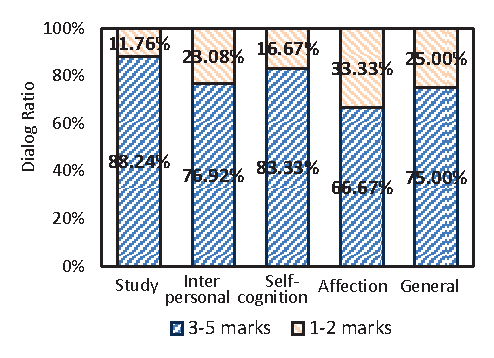
\includegraphics[width=5.5cm]{figs/experimentresult.eps}
\caption{5 stress categories mark distribution}
\label{fig:score}
\end{minipage}
\makeatletter\def\@captype{table}\makeatother
\begin{minipage}{.45\textwidth}
\centering
\caption{Accuracy of stress detection}
\begin{tabular}{c|c|c}
\hline
 &Precision&Recall
\\\hline
 \multicolumn{3}{l}{Accuracy of stress existence detection}
\\\hline
Stress &73.15\%&63.37\%
\\\hline
No stress&83.53\%&88.87\%
\\\hline
Average&78.34\%&76.12\%
\\\hline
 \multicolumn{3}{l}{Accuracy of stress category detection}
\\\hline
Study&86.20\%&75.00\%
\\\hline
Self-Cognition&93.90\%&46.27\%
\\\hline
Inter-Personal&53.84\%&76.56\%
\\\hline
Affection&82.05\%&42.60\%
\\\hline
General&30.94\%&76.92\%
\\\hline
Average&69.39\%&63.47\%
\\\hline
\end{tabular}
\label{tab:stress_detection}
\end{minipage}
\end{figure}
\begin{table}
 \caption{Conversation distribution  of the change mode about stressful sentence ratio}
\centering
\begin{tabular}{c|c|c|c|c|c|c}
\hline
&\multicolumn{2}{|c|}{Change mode}&Freq&Perc&Freq\_sum&Perc\_sum
\\\cline{2-3}
%\\\hline
 &Early-Middle &Middle-Late  &&&&
\\\hline
 &$\downarrow$&$\downarrow$&17&27.42\%&&
\\\cline{2-5}
Effective&$\rightarrow$&$\downarrow$&7&11.29\%&&
\\\cline{2-5}
&$\uparrow$&$\downarrow$&8&12.90\%&45&72.58\%
\\\cline{2-5}
&$\downarrow$&$\rightarrow$&13&20.97\%&&
\\\hline
&$\downarrow$&$\uparrow$&7&11.29\%&&
\\\cline{2-5}
&$\rightarrow$&$\uparrow$&0&0.00\%&&
\\\cline{2-5}
Ineffective&$\rightarrow$&$\rightarrow$&6&9.68\%&17&27.42\%
\\\cline{2-5}
&$\uparrow$&$\rightarrow$&3&4.84\%&&
\\\cline{2-5}
&$\uparrow$&$\uparrow$&1&1.61\%&&
\\\hline
\end{tabular}
%}
\label{tab:changemode}
\end{table}

\textit{The change of users stress status according to Chinese CPSS.}
\begin{table}
 \caption{Number of people of 3 kinds of stress status evolving type}
\centering
\begin{tabular}{c|c|c|c|c}
\hline
 &Improved&Not change&Deteriorated&Total
\\\hline
 Week 1&2&0&8&10
\\\hline
Week 2&5&1&4&10
\\\hline
Week 3&5&1&4&10
\\\hline
Week 4&7&1&2&10
\\\hline
\end{tabular}
\label{tab:CPSS}
\end{table}
For each user, we asked them to fill the Chinese CPSS questionnaire to record the evolving of their stress status. In the questionnaire, higher score represents heavier stress. We consider that score decreasing means the stress status has been improved, score increasing means the stress status has deteriorated. Table~\ref{tab:CPSS} shows that more and more users were feeling better as time goes by.
